\documentclass[11pt]{article}
\usepackage[utf8]{inputenc}
\usepackage[T1]{fontenc}
\usepackage{amsmath}
\usepackage{amssymb} % Needed for \eth if used
\usepackage{graphicx}
\usepackage{geometry}
\usepackage{tikz}
\usepackage{pgfplots} % For plots
\usepackage{ulem}     % For underline, using normalem to avoid messing with \emph

\geometry{a4paper, margin=1in}
\usetikzlibrary{positioning, arrows.meta, shapes.geometric} % For TikZ diagrams
\pgfplotsset{compat=1.18} % Use a recent PGFPlots version

% Custom commands (optional)
\newcommand{\avg}[1]{\overline{#1}}
\newcommand{\prob}[1]{P(#1)}
\newcommand{\ProbDens}[1]{\mathcal{P}(#1)} % Using script P for density
\newcommand{\vect}[1]{\vec{#1}}
\newcommand{\dd}[1]{\mathrm{d}#1} % Differential d
\newcommand{\pderiv}[2]{\frac{\partial #1}{\partial #2}}
\newcommand{\deriv}[2]{\frac{\mathrm{d} #1}{\mathrm{d} #2}}
\newcommand{\muState}{\mu\text{-state}} % Microstate
\newcommand{\OmegaE}{\Omega(E)}
\newcommand{\omegaE}{\omega(E)}
\newcommand{\PhiE}{\Phi(E)}
\newcommand{\deltaE}{\delta E}
\newcommand{\ethbar}{\text{\it{đ}}} % \eth symbol for inexact differential
\newcommand{\kb}{k_B} % Boltzmann constant
\newcommand{\tE}{\tilde{E}} % Most probable energy

\title{Physics 415 - Lecture 8: Entropy and Equilibrium}
\date{February 7, 2025}
\author{} % Author not specified

\begin{document}

\maketitle
\thispagestyle{empty}

\section*{Summary of Lecture 7}

\begin{itemize}
    \item $\OmegaE = \#$ accessible states with energy $(E, E+\deltaE)$.
    \item Entropy: $S = \ln \Omega$. (Dimensionless definition for now).
    \item Temperature: $\frac{1}{T} = \pderiv{S}{E}$. ($T$ has units of energy).
    \item $S$ and $T$ are functions of the macrostate of the system.
    \item Thermal interaction between systems 1 and 2 (isolated together, $E=E_1+E_2=$ const):
    \begin{center}
    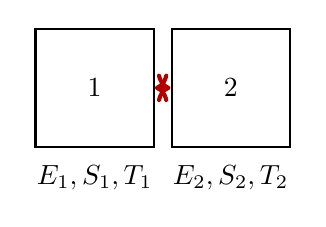
\begin{tikzpicture}
        \node (A) [draw, thick, minimum width=1.5cm, minimum height=1.5cm, label=center:1] {};
        \node (B) [draw, thick, minimum width=1.5cm, minimum height=1.5cm, right=0.2cm of A, label=center:2] {};
        \draw [line width=1.5pt, red!70!black, <->] (A.east) -- (B.west);
        \node at (A.south) [below=0.1cm] {$E_1, S_1, T_1$};
        \node at (B.south) [below=0.1cm] {$E_2, S_2, T_2$};
    \end{tikzpicture}
    \end{center}
    \item Probability $P_1(E_1)$ is sharply peaked at $E_1 = \tE_1$. Width $\Delta^* E_1 \ll \tE_1$.
    \begin{center}
    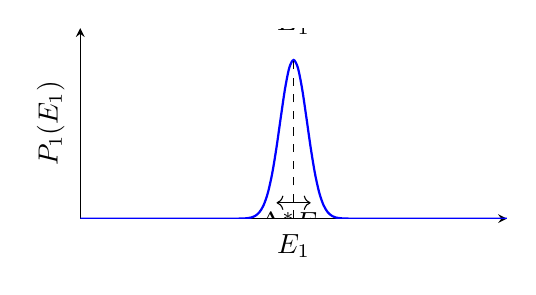
\begin{tikzpicture}
    \begin{axis}[
        axis lines=left, xlabel=$E_1$, ylabel=$P_1(E_1)$,
        xtick=\empty, ytick=\empty, ymax = 1.2, samples=101, smooth,
        width=7cm, height=4cm
    ]
    \addplot [domain=0:5, thick, blue] {exp(-20*(x-2.5)^2)}; % Sharper peak
    \draw [dashed] (axis cs:2.5, 0) -- (axis cs:2.5, 1) node[pos=1.1, above] {$\tE_1$};
    \draw [<->] (axis cs:2.3, 0.1) -- (axis cs:2.7, 0.1) node[midway, below] {$\Delta^* E_1$};
    \end{axis}
    \end{tikzpicture}
    \end{center}
    \item Condition for maximum probability ($E_1=\tE_1$) is $S_{tot} = S_1 + S_2 = \text{max}$.
    \item This implies the equilibrium condition: $T_1 = T_2$. The most probable state has equal temperatures.
    \item If initially $E_1 = E_1^{(0)} \neq \tE_1$ and $E_2 = E_2^{(0)} \neq \tE_2$, the system evolves towards the most probable state $(\tE_1, \tE_2)$.
    \item During this spontaneous process for an isolated system (1+2), the total entropy increases:
    \[ \Delta S_{tot} = S_{tot}(\text{final}) - S_{tot}(\text{initial}) = [S_1(\tE_1) + S_2(\tE_2)] - [S_1(E_1^{(0)}) + S_2(E_2^{(0)})] \ge 0 \]
\end{itemize}

\section*{Tying up Loose Ends}

\subsection*{Dependence of Entropy $S$ on Energy Range $\deltaE$}

We defined $S = \ln \OmegaE$. Since $\OmegaE = \omegaE \deltaE$, where $\omegaE$ is the density of states (independent of $\deltaE$), we have:
\[ S = \ln(\omegaE \deltaE) = \ln \omegaE + \ln \deltaE \]
So the entropy $S$ formally depends on the choice of $\deltaE$.
If we choose a different subdivision $\deltaE'$, the entropy would be $S' = \ln(\omegaE \deltaE')$.
The difference is $S - S' = \ln(\deltaE / \deltaE')$.

However, for macroscopic systems, $S \sim N$ (\# of DOF or particles, $N \sim 10^{23}$).
The term $\ln(\deltaE / \deltaE')$ is just a constant, independent of $N$, and utterly negligible compared to $S \sim N$.
Even if $\deltaE' \sim N \deltaE$, $\ln(1/N) \sim -\ln N \ll N$.
Conclusion: For $N \gg 1$, the choice of $\deltaE$ does not affect macroscopic results. $S \approx S'$ for all practical purposes.

Note also that the temperature $T$ is independent of $\deltaE$:
\[ \frac{1}{T} = \pderiv{S}{E} = \pderiv{}{E} (\ln \omegaE + \ln \deltaE) = \pderiv{(\ln \omegaE)}{E} \]

\subsection*{Additivity Property of Entropy}

Consider the combined system 1+2 in thermal equilibrium ($T_1=T_2$).
The total number of states is $\Omega(E) = \sum_{E_1} \Omega_1(E_1) \Omega_2(E-E_1)$.
Let $S = \ln \Omega$, $S_1 = \ln \Omega_1$, $S_2 = \ln \Omega_2$.

As discussed, the probability $P_1(E_1) = \Omega_1(E_1)\Omega_2(E-E_1)/\Omega(E)$ is sharply peaked around $E_1 = \tE_1$ with width $\Delta^* E_1$.
The sum for $\Omega(E)$ is dominated by terms near the peak:
\[ \Omega(E) \approx \sum_{E_1 \in (\tE_1 \pm \Delta^* E_1)} \Omega_1(E_1) \Omega_2(E-E_1) \]
Approximating the term $\Omega_1(E_1)\Omega_2(E-E_1)$ by its maximum value $\Omega_1(\tE_1)\Omega_2(\tE_2)$ over the width of the peak $\Delta^* E_1$. The number of terms in the sum is roughly $\Delta^* E_1 / \delta E$ (where $\delta E$ is the energy step size, related to the cell size used for $\Omega$).
\[ \Omega(E) \approx [\Omega_1(\tE_1) \Omega_2(\tE_2)] \times (\text{\# of states in peak}) \approx [\Omega_1(\tE_1) \Omega_2(\tE_2)] \times \frac{\Delta^* E_1}{\delta E} \]
Taking the logarithm:
\[ S = \ln \Omega \approx \ln \Omega_1(\tE_1) + \ln \Omega_2(\tE_2) + \ln\left(\frac{\Delta^* E_1}{\delta E}\right) \]
\[ S \approx S_1(\tE_1) + S_2(\tE_2) + \ln\left(\frac{\Delta^* E_1}{\delta E}\right) \]
The first two terms $S_1, S_2$ scale with $N_1, N_2$ respectively ($\sim N$).
The last term involves the width $\Delta^* E_1 \sim \tE_1/\sqrt{N_1}$ and $\delta E$. The ratio $\Delta^* E_1 / \delta E$ might be large, but its logarithm $\ln(\dots)$ scales at most as $\ln N$ or is independent of $N$.
This logarithmic term will always be negligible compared to $S_1+S_2$ (which scale as $N$) for macroscopic systems ($N \gg 1$).

Therefore, for macroscopic systems ($N \gg 1$):
\[ S \approx S_1 + S_2 \]
The entropy of the combined system (at equilibrium) is the sum of the individual entropies (evaluated at the most probable energies $\tE_1, \tE_2$). Entropy is additive (extensive). This is similar to the total energy $E=E_1+E_2$.

\section*{Sharpness of the Probability Distribution}

Let's analyze $P_1(E_1)$ near its maximum $\tE_1$. Write $E_1 = \tE_1 + \eta$, where $\eta$ is small.
We expand $\ln P_1(E_1) = \ln \Omega_1(E_1) + \ln \Omega_2(E_2) - \ln \Omega(E)$ around $\eta=0$.
Recall $E_2 = E-E_1 = (E-\tE_1) - \eta = \tE_2 - \eta$.
Using Taylor expansion for $S = \ln \Omega$:
\[ S_1(\tE_1 + \eta) = S_1(\tE_1) + \left.\pderiv{S_1}{E_1}\right|_{\tE_1} \eta + \frac{1}{2} \left.\pderiv[2]{S_1}{E_1}\right|_{\tE_1} \eta^2 + \dots \]
\[ S_2(\tE_2 - \eta) = S_2(\tE_2) + \left.\pderiv{S_2}{E_2}\right|_{\tE_2} (-\eta) + \frac{1}{2} \left.\pderiv[2]{S_2}{E_2}\right|_{\tE_2} (-\eta)^2 + \dots \]
Let $1/T_1 = (\partial S_1/\partial E_1)|_{\tE_1}$ and $1/T_2 = (\partial S_2/\partial E_2)|_{\tE_2}$. At equilibrium, $T_1=T_2=T$.
Define curvature parameters:
\[ \lambda_1 \equiv - \left.\pderiv[2]{S_1}{E_1}\right|_{\tE_1} = - \left.\pderiv{(1/T_1)}{E_1}\right|_{\tE_1} \]
\[ \lambda_2 \equiv - \left.\pderiv[2]{S_2}{E_2}\right|_{\tE_2} = - \left.\pderiv{(1/T_2)}{E_2}\right|_{\tE_2} \]
For the sum $S_1+S_2$ to be maximum at $\eta=0$, we need the second derivative to be negative, so $\lambda_1 > 0$ and $\lambda_2 > 0$.
Then:
\[ S_1(\tE_1 + \eta) + S_2(\tE_2 - \eta) \approx S_1(\tE_1) + S_2(\tE_2) + \left(\frac{1}{T_1} - \frac{1}{T_2}\right)\eta - \frac{1}{2}(\lambda_1 + \lambda_2)\eta^2 \]
Since $T_1=T_2=T$ at the maximum (equilibrium):
\[ S_1(E_1) + S_2(E_2) \approx S_1(\tE_1) + S_2(\tE_2) - \frac{1}{2}\lambda \eta^2 \]
where $\lambda = \lambda_1 + \lambda_2 > 0$.
Now, $\ln P_1(E_1) = (S_1(E_1) + S_2(E_2)) - \ln \Omega(E)$.
Since $\ln P_1(\tE_1) = (S_1(\tE_1) + S_2(\tE_2)) - \ln \Omega(E)$, we have:
\[ \ln P_1(E_1) \approx \ln P_1(\tE_1) - \frac{1}{2}\lambda \eta^2 \]
\[ \implies P_1(E_1) \approx P_1(\tE_1) e^{-\frac{1}{2}\lambda \eta^2} = P_1(\tE_1) e^{-(E_1-\tE_1)^2 / (2 \lambda^{-1})} \]
This is a Gaussian distribution for the energy $E_1$ around its most probable (and mean) value $\tE_1$.
The width of the distribution (standard deviation) is:
\[ \Delta^* E_1 \equiv \frac{1}{\sqrt{\lambda}} = \frac{1}{\sqrt{\lambda_1 + \lambda_2}} \]
For $|E_1 - \tE_1| > \Delta^* E_1$, the probability is negligible.

\textbf{Estimate of the width $\Delta^* E_1$:}
We had $S_1 \sim a_1 N_1 \ln E_1$.
$\pderiv{S_1}{E_1} \sim \frac{a_1 N_1}{E_1} = \frac{1}{T_1}$.
$\pderiv[2]{S_1}{E_1} \sim - \frac{a_1 N_1}{E_1^2} = -\lambda_1$. So $\lambda_1 \sim N_1/E_1^2$ (since $a_1 \sim O(1)$).
The width $\Delta^* E_1 = (\lambda_1 + \lambda_2)^{-1/2}$. If system 1 is much smaller than system 2 ($N_1 \ll N_2$), then typically $\lambda_1 \gg \lambda_2$ , or consider combined system. Let's assume $\lambda \sim N/E^2$ where $N=N_1+N_2$ and $E=E_1+E_2$.
Then $\Delta^* E_1 \sim \sqrt{E^2/N} = E/\sqrt{N}$.
Let's refine using $\lambda_1 \sim N_1/E_1^2$. If $N_1 \sim N$, $E_1 \sim E$, then $\lambda \sim N/E^2$.
The width scales as $\Delta^* E_1 \sim E/\sqrt{N}$.
The relative width is:
\[ \frac{\Delta^* E_1}{\tE_1} \sim \frac{E/\sqrt{N}}{E/N} \sim \frac{1}{\sqrt{N}} \]
(Assuming $E_1 \propto N_1 \propto N$).
Since $N$ is macroscopic ($N \sim 10^{23}$), $\sqrt{N} \sim 10^{11.5}$. The relative width $1/\sqrt{N}$ is extremely small.
Fluctuations about the mean (most probable) value are utterly negligible.

\textbf{Conclusion:} This behavior is generic for macroscopic quantities (energy, pressure, etc.). They are essentially equal to their most probable (=mean) values. Even though our $\mu$-scopic description is statistical, the predictions for macroscopic behavior are essentially deterministic because statistical fluctuations are so insignificant.

\textbf{Also note:} $\lambda = - \partial^2 S / \partial E^2 = - \partial(1/T)/\partial E = - (-\frac{1}{T^2}) \pderiv{T}{E} = \frac{1}{T^2} \pderiv{T}{E}$.
Since $\lambda > 0$ (for stability/maximum) and $T^2 > 0$, we must have $\pderiv{T}{E} > 0$.
The temperature $T$ of a typical macroscopic system is an increasing function of its energy $E$.

\section*{Reversible and Irreversible Processes}

Entropy leads to the concept of "reversible" and "irreversible" processes.
\begin{itemize}
    \item For systems in thermal contact (isolated together), the total entropy increases as equilibrium is approached: $\Delta S_{tot} = \Delta S_1 + \Delta S_2 \ge 0$.
    \item In general, when a constraint on a closed/isolated system is removed, the entropy can only increase or stay the same. $\Delta S_{isolated} \ge 0$. (This is the Second Law of Thermodynamics).
    \item A process is "irreversible" if the total entropy of the isolated system involved increases ($\Delta S > 0$).
        \textbf{Example:} Heat transfer between two bodies initially at different temperatures $T_1^{(0)} \neq T_2^{(0)}$. When they reach equilibrium at $T_f = T_1 = T_2$, the final total entropy $S_f = S_1(\tE_1) + S_2(\tE_2)$ is greater than the initial total entropy $S^{(0)} = S_1(E_1^{(0)}) + S_2(E_2^{(0)})$.
    \item A process is "reversible" if the total entropy of the isolated system involved remains constant ($\Delta S = 0$). These processes must proceed quasi-statically through a sequence of equilibrium states. (Examples later).
\end{itemize}

\end{document}